%=======================================================================
\section{The Feature Descriptors in Detail}

This section explains what each descriptor measures, the clinical intuition behind it, the parameters that
control its behaviour, and the size of the feature vector it produces in this project.

%----------------------------------------------------------------------
\subsection{GLCM --- Gray-Level Co-occurrence Matrix}
\textbf{Idea.} GLCM is the classic Haralick texture descriptor. It counts how often a pixel of gray
level $i$ appears at a fixed offset (distance + direction) from a pixel of gray level $j$. The result
is a co-occurrence matrix $P(i,j)$ that summarises the spatial relationship between intensities ---
i.e.\ the \textbf{texture} of the tissue. Tumor types differ heavily in how smooth, coarse, or directional
their texture is. For instance, necrotic cores in glioblastomas often exhibit vastly different localized 
homogeneity compared to the surrounding edema, which GLCM captures exceptionally well.

\documentclass{article}
\usepackage{tikz}
\usetikzlibrary{shapes.geometric, arrows.meta, positioning, calc}

\begin{document}

\begin{figure}[hbt!]
\centering
\begin{tikzpicture}[
    node distance=1.5cm and 2.0cm, 
    scale=0.9, 
    every node/.style={transform shape},
    % Define clean, unified styles for the pipeline steps
    block/.style={draw, fill=blue!5, border width=1pt, minimum width=2.8cm, minimum height=2.5cm, align=center, rounded corners=6pt, font=\small},
    featblock/.style={draw, fill=gray!5, border width=1pt, minimum width=2.8cm, minimum height=2.5cm, align=left, rounded corners=6pt, font=\small\sffamily, inner sep=10pt},
    arrow/.style={-{Stealth[scale=1.2]}, thick, color=black!70}
]
  
  % Step 1: Input Image Matrix
  \node (img) [block] {\textbf{Image Matrix}\\[0.5em] $I(x,y)$};
  
  % Step 2: GLCM Matrix
  \node (glcm) [block, right=of img] {\textbf{GLCM Matrix}\\[0.5em] $P(i,j)$};
  
  % Step 3: Texture Features
  \node (feat) [featblock, right=of glcm] {
    $\bullet$ Contrast \\
    $\bullet$ Correlation \\
    $\bullet$ Energy \\
    $\bullet$ Homogeneity \\
    $\bullet$ \dots
  };
  
  % Standardized, perfectly spaced arrows using the relative positions
  \draw[arrow] (img) -- (glcm) 
    node[midway, above=1pt, font=\footnotesize\bfseries] {$(d, \theta)$} 
    node[midway, below=1pt, font=\footnotesize, text=gray] {Offset};
    
  \draw[arrow] (glcm) -- (feat) 
    node[midway, above=1pt, font=\footnotesize\bfseries] {Extract} 
    node[midway, below=1pt, font=\footnotesize, text=gray] {Moments};

\end{tikzpicture}
\caption{The GLCM extraction pipeline: mapping pixel spatial co-occurrences at a specified distance ($d$) and angle ($\theta$) to statistical texture features.}
\label{fig:glcm_pipeline}
\end{figure}

\end{document}


\textbf{What we compute.} From each normalised co-occurrence matrix we extract six standard Haralick
properties and average them over all distance/angle pairs:
\begin{itemize}[leftmargin=1.4em,itemsep=1pt]
  \item \textbf{Contrast} --- local intensity variation (high for coarse, heterogeneous texture).
  \item \textbf{Dissimilarity} --- like contrast but grows linearly with intensity differences.
  \item \textbf{Homogeneity} --- how close $P(i,j)$ mass sits to the diagonal (high for smooth, uniform regions).
  \item \textbf{Energy / ASM} --- textural uniformity (Angular Second Moment and its square root).
  \item \textbf{Correlation} --- linear dependency of gray levels at the given spatial offset.
\end{itemize}

\textbf{Parameters tuned.}
\begin{center}
\begin{tabularx}{\textwidth}{@{}l Y Y@{}}
\toprule
\thd{Parameter} & \thd{Meaning} & \thd{Effect} \\
\midrule
distances  & Pixel offsets at which co-occurrence is measured & Small $=$ fine texture; large $=$ coarse structure \\
angles     & Directions (radians) of the offset & Captures directional vs.\ isotropic texture \\
levels     & Number of gray-level bins & Higher $=$ finer detail but noisier / sparser matrix \\
symmetric  & Average $P(i,j)$ with $P(j,i)$ & Makes the descriptor direction-agnostic \\
\bottomrule
\end{tabularx}
\end{center}
\textbf{Output size:} 6 features (always), regardless of parameters, because only the six averaged
properties are kept.

%----------------------------------------------------------------------
\subsection{LBP --- Local Binary Patterns}
\textbf{Idea.} LBP describes \textbf{micro-texture}. For every pixel, it looks at $P$ neighbours on a
circle of radius $R$, thresholds each neighbour against the centre pixel (1 if brighter, 0 otherwise),
and reads the bits as a binary code. The histogram of these codes over the whole image is the feature
vector. In neuro-oncology, varying cell densities and micro-vascular proliferation present as 
micro-textural variations. Because LBP relies purely on relative intensity differences, it is 
\textbf{invariant to monotonic gray-scale changes} (making it highly robust to MRI bias field artifacts) 
and is extremely cheap to compute.

\begin{figure}[hbt!]
\centering
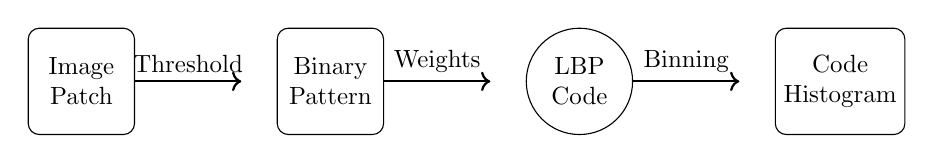
\begin{tikzpicture}[node distance=1.5cm, scale=0.9, every node/.style={transform shape}]
  \node (patch) [draw, minimum width=1.5cm, minimum height=1.5cm, align=center, rounded corners] {Image\\Patch};
  \draw[->, thick] (patch.east) -- ++(1.5,0) node[midway, above] {Threshold};
  \node (binary) [draw, minimum width=1.5cm, minimum height=1.5cm, align=center, right=of patch, xshift=0.5cm, rounded corners] {Binary\\Pattern};
  \draw[->, thick] (binary.east) -- ++(1.5,0) node[midway, above] {Weights};
  \node (value) [draw, circle, minimum size=1.5cm, align=center, right=of binary, xshift=0.5cm] {LBP\\Code};
  \draw[->, thick] (value.east) -- ++(1.5,0) node[midway, above] {Binning};
  \node (hist) [draw, minimum width=1.5cm, minimum height=1.5cm, align=center, right=of value, xshift=0.5cm, rounded corners] {Code\\Histogram};
\end{tikzpicture}
\caption{The LBP computation process: converting local pixel neighbourhoods into discrete binary codes to build a micro-texture histogram.}
\label{fig:lbp_pipeline}
\end{figure}

\textbf{Parameters tuned.}
\begin{center}
\begin{tabularx}{\textwidth}{@{}l Y Y@{}}
\toprule
\thd{Parameter} & \thd{Meaning} & \thd{Effect} \\
\midrule
$P$    & Number of sampling points on the circle & More points $=$ finer texture, longer histogram \\
$R$    & Radius of the neighbourhood (pixels)    & Larger $=$ captures coarser texture \\
method & LBP variant: uniform / nri\_uniform / ror & Controls rotation-invariance \& histogram length \\
\bottomrule
\end{tabularx}
\end{center}
The \texttt{uniform} and \texttt{nri\_uniform} variants keep only patterns with $\leq 2$
bit-transitions, giving a compact $P{+}2$-bin histogram that is robust to noise; \texttt{ror} is
rotation-invariant but denser. Histograms are normalised to a probability distribution so image size
does not affect the values.

\textbf{Output size:} $P+2$ bins for the uniform methods (so the selected configuration produces
\textbf{10 features}).

%----------------------------------------------------------------------
\subsection{DWT --- Discrete Wavelet Transform}
\textbf{Idea.} The DWT decomposes an image into \textbf{frequency sub-bands at multiple scales}. A
2-D wavelet transform splits the image into an approximation band (LL --- coarse content) and three
detail bands (LH, HL, HH --- horizontal, vertical, and diagonal edges). Applying it repeatedly to the
LL band gives a multi-resolution pyramid. This is critical because pathological features manifest at 
varying scales: coarse bands capture the overall tumor bulk and shape, while detail bands encode fine, 
directional tissue irregularities.

\begin{figure}[hbt!]
\centering
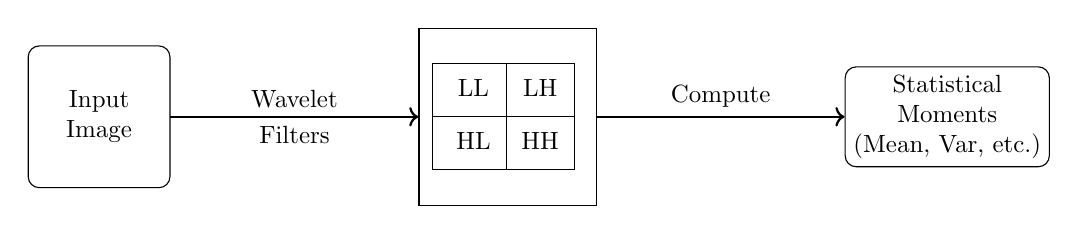
\begin{tikzpicture}[node distance=1.5cm, scale=0.9, every node/.style={transform shape}]
  \node (input) [draw, minimum width=2cm, minimum height=2cm, align=center, rounded corners] {Input\\Image};
  \node (bands) [draw, minimum width=2.5cm, minimum height=2.5cm, align=center, right=of input, xshift=2cm] {
    \begin{tabular}{|c|c|}
    \hline
    \rule{0pt}{3ex} LL & LH \\[1ex] \hline
    \rule{0pt}{3ex} HL & HH \\[1ex] \hline
    \end{tabular}
  };
  \draw[->, thick] (input.east) -- (bands.west) node[midway, above] {Wavelet} node[midway, below] {Filters};
  \node (stats) [draw, right=of bands, xshift=2cm, align=center, rounded corners] {Statistical\\Moments\\(Mean, Var, etc.)};
  \draw[->, thick] (bands.east) -- (stats.west) node[midway, above] {Compute};
\end{tikzpicture}
\caption{The 2D Discrete Wavelet Transform (Level 1) decomposing an image into four frequency sub-bands, followed by statistical pooling.}
\label{fig:dwt_pipeline}
\end{figure}

\textbf{What we compute.} Rather than keep the (large) coefficient images, we summarise every
sub-band with four statistics: \textbf{mean, standard deviation, energy (mean of squares), and
entropy}. A level-$L$ decomposition has $3L+1$ sub-bands, giving $4\times(3L+1)$ features.

\textbf{Parameters tuned.}
\begin{center}
\begin{tabularx}{\textwidth}{@{}l Y Y@{}}
\toprule
\thd{Parameter} & \thd{Meaning} & \thd{Effect} \\
\midrule
wavelet & Wavelet family (haar, db2, db4, sym2 \dots) & Sets smoothness \& symmetry of the basis \\
level   & Decomposition depth & More levels $=$ coarser bands, more features \\
\bottomrule
\end{tabularx}
\end{center}
\textbf{Output size:} $4\times(3\cdot\text{level}+1)$. The selected configuration (level 1) produces
\textbf{16 features}.

%----------------------------------------------------------------------
\subsection{HOG --- Histogram of Oriented Gradients}
\textbf{Idea.} HOG describes \textbf{local shape and edge structure}. The image is divided into small
cells; within each cell, a histogram of gradient orientations (weighted by gradient magnitude) is
built; cells are grouped into blocks and normalised for contrast invariance. The concatenation of all
block histograms forms the feature vector. This makes HOG particularly sensitive to morphological 
boundaries. A sharply circumscribed benign lesion will yield highly concentrated directional gradients, 
whereas an aggressively infiltrating malignancy will produce chaotic, multi-directional histograms.

\begin{figure}[hbt!]
\centering
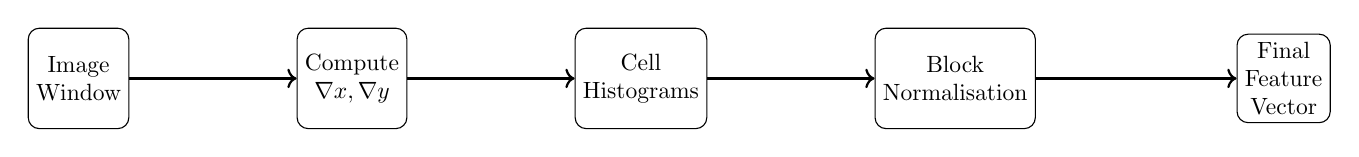
\begin{tikzpicture}[node distance=1.5cm, scale=0.85, every node/.style={transform shape}]
  \node (img) [draw, minimum width=1.5cm, minimum height=1.5cm, align=center, rounded corners] {Image\\Window};
  \node (grad) [draw, minimum width=1.5cm, minimum height=1.5cm, align=center, right=of img, xshift=1cm, rounded corners] {Compute\\$\nabla x, \nabla y$};
  \node (cells) [draw, minimum width=1.5cm, minimum height=1.5cm, align=center, right=of grad, xshift=1cm, rounded corners] {Cell\\Histograms};
  \node (blocks) [draw, minimum width=1.5cm, minimum height=1.5cm, align=center, right=of cells, xshift=1cm, rounded corners] {Block\\Normalisation};
  \node (concat) [draw, right=of blocks, xshift=1.5cm, align=center, rounded corners] {Final\\Feature\\Vector};

  \draw[->, thick] (img.east) -- (grad.west);
  \draw[->, thick] (grad.east) -- (cells.west);
  \draw[->, thick] (cells.east) -- (blocks.west);
  \draw[->, thick] (blocks.east) -- (concat.west);
\end{tikzpicture}
\caption{The HOG extraction pipeline: moving from spatial gradients to contrast-normalised directional histograms.}
\label{fig:hog_pipeline}
\end{figure}

\textbf{Parameters tuned.}
\begin{center}
\begin{tabularx}{\textwidth}{@{}l Y Y@{}}
\toprule
\thd{Parameter} & \thd{Meaning} & \thd{Effect} \\
\midrule
orientations    & Number of gradient-direction bins & More bins $=$ finer angular resolution \\
pixels\_per\_cell & Spatial size of each cell        & Smaller $=$ more detail, much longer vector \\
cells\_per\_block & Block size for normalisation     & Controls contrast-normalisation neighbourhood \\
block\_norm     & Normalisation scheme (L2-Hys)      & Robustness to local contrast changes \\
\bottomrule
\end{tabularx}
\end{center}
\textbf{Output size:} depends on cell/block geometry; the selected configuration produces
\textbf{1{,}176 features} --- by far the largest branch, which is why feature cleaning later matters
most for HOG.